\chapter[\'Etude en clinique]{\'Etude avec utilisation du test
  d'écoute en clinique psychiatrique}

Nous savons que la musicothérapie est de plus en plus intégrée dans
les milieux psychiatriques.
L'objectif ici est de vérifier l'hypothèse évoquée plus haut qui est celle de
savoir s'il est possible de mesurer, après un travail 
musicothérapeutique, la transformation de l'écoute chez le
patient.
Les tests ont été faits en avril, mai, juin, juillet, septembre et octobre 2017.

\section{Cadre de travail}

 La Privatklinik
de Meiringen est  spécialisée en
addictologie dans le canton de Berne. Elle dispose d'une capacité de 195 lits, 33 médecins et
psychologues, secondés par 177 soignants qui assurent les soins du
patient.




\subsection{Les patients: description}


 \begin{itemize}
 
 \item Nbre: 29 personnes, dont 19 hommes et 10 femmes, de 25 - 72
   ans, x=

   Tableau à faire...moyenne des âges 
 

 \item Pathologies:  burnout, dépendances, dépression.

 \item Temps de séjour: 3 à 6 semaines, voire plusieurs mois. Ici, pour
notre étude , nous avons choisi de prendre la période de 3 semaines
qui correspond à la durée moyenne.
 \item Fréquence du traitement en musicothérapie: 1x par semaine pendant
50mn à 60mn.
 \item Le type de musicothérapie: réceptif ou actif, adapté selon les pathologies.
 \item Ont été  exclus l'écoute avec casques et  musiques traitées
   chez Tomatis.
 \item Contexte de la clinique: habituel pour une prise en
charge en clinique psychiatrique 
par les médecins, psychiatres, psychologues et thérapeutes.
Nous citerons les diverses thérapies proposées: physio--,ergo--,
art--,musico--,corporel--, zoo--  (chien/ cheval)  ainsi
que par les  ateliers de créativité sur le bois, la terre, la laine.  

\end{itemize}
\section{Design d'étude}

Mise en place:

Un groupe d'intervention (GI) et un groupe de contrôle (GC) ont été constitués.
La direction de la clinique ayant accepté l'étude, le personnel soignant et tout le
corpus des thérapies créatives ont  été
informés au préalable.
Une feuille explicative de l'étude sur  l'évaluation de l'écoute et
sur
l'hypothèse de sa transformation lors d'un 
séjour en thérapie. \emph{Information für Mitwirkende an der klinischen
  Studie\  ``Evaluierung des aktiven Hörvermögens" } a été diffusée pour informer les patients.
Ceux-ci ont été aussi avertis par un
court entretien individuel réalisé généralement par la musicothérapeute Regula Lehman  \footnote{Regula
  Lehmann, musicothérapeute  à 90\%  à la clinique de Meiringen.}.

Les patients étaient libres de participation. Ceux qui
l'ont fait, ont signé leur accord  officiellement à chaque fois  \emph{``Eine schriftliche Einbewilligung zum
  Test"}.

\paragraph{Les groupes}

Le groupe GI, d'intervention, a comporté finalement 21 patients, avec 15 hommes et 6
femmes.
Le groupe GC a comporté 8 patients, 4 hommes et 4 femmes.

Nous avions prévu 10 pour chaque groupe au départ. Nous avons
constaté la grande 
variabilité due soit aux sorties prématurées, à des rendez-vous chez le médecin
ou de l'incapacité physique/psychique de certains patients à venir. De
ce fait,
nous avons accepté que certains patients passent le test lorsqu'ils le
demandaient,même s'ils
n'étaient pas prévus. C'est l'intérêt des patients pour l'appareil
test dans la salle de musicothérapie qui a suscité des questions et
l'envie de tenter l'expérience. C'est pour cela que nous expliquons
cette différence de participation.

 
 
 

\section{Instruments de mesure: le WHO QOL - Bref et le test d'écoute}
 Nous redonnons quelques précisions sur le WHO QOL-Bref mais ne
 reviendrons pas sur le test d'écoute, suffisamment décrit au chapitre 8.

 \subsection{Le WHO QOL - Bref}
 
Le  WHOQOL-Bref sert à évaluer la qualité de vie des patients. C'est une échelle
d'auto-évaluation subjective qui évalue la santé mentale, le
bien-être, l'environnement et les relations sociales.
Il s'agit ici de la version courte  la plus récente (2004) du questionnaire
 WHOQOL-100 datant de 1998, version issue du Programme sur la santé
 mentale de l'
Organisation mondiale de la santé de Genève. Il y a 26 questions
courtes, dont un item concernant la qualité de vie globale
auto-évaluée par le sujet, un item évaluant la santé générale perçue
et les 24 autres se répartissent selon les 4 domaines suivants:  
: physique, psychologique, relations sociales et environnement.
\begin{enumerate}
	\item  Le domaine de la perception physique (7 items) comprend l' activité quotidienne// la dépendance et/ou l'assistance médicale// la fatigabilité, l'énergie//la mobilité// la douleur// le sommeil// la capacité de travail//
	
		 \item Le domaine psychologique (6 items):  image de soi, apparence// ressentis positifs et négatifs// estime de soi// spiritualité, croyances personnelles, religion// mémoire et concentration, apprentissage, pensée.
		
			\item Le domaine des relations sociales (3 items) : relations personnelles// soutien social// vie sexuelle.
			
			\item Le domaine de l'environnement (8 items) :
                          l'environnement domestique et physique
                          (pollution, bruit, trafic, climat)// la
                          situation financière//  la liberté, la
                          sécurité physique et morale//
                          l'accessibilité et qualité de la santé// les
                          opportunités de détente, loisirs, accès aux
                          informations// logement et transport// 
		\end{enumerate}
		
	

Les questions varient selon sa propre perception, telle la satisfaction
au sujet de son  sommeil, de sa vie relationelle, sexuelle, de
l'opinion de que l'on a sur soi,  `` Êtes-vous satisfait de
vous-même?'' , ``Acceptez-vous votre apparence physique?''ou si le patient éprouve souvent des sentiments négatifs
et/ou s'il a assez d'énergie dans la vie de tous les jours.
La cotation se fait sur 4 types d'échelles de réponses en 5 points
permettant l'évaluation de l'intensité, la fréquence, la capacité, l'évaluation.
de 1 à 5.
Le patient le remplit avec ou sans aide du
thérapeut lors de chaque test
d'écoute. La durée variera de 3 à 10 minutes en
moyenne. 
Nous avons utilisé et fait en parallèle le test WHOQO-Bref pour avoir une variable supplémentaire pour confirmer en
parallèle supposée de l'action de la musicothérapie sur une éventuelle modification de l'écoute.


        	
        \subsection{Technique d'intervention:}


       
\begin{itemize}
	\item Le groupe GI de patients en musicothérapie : un
          test avant leur prise en charge en musicothérapie; avec un questionnaire
          WHOQOL.
          
          \item Un 2\ieme\ test et un questionnaire WHOQOL : après 4 semaines de
          clinique.
          
	\item Un groupe GC de contrôle sans musicothérapie,
	toujours dans le même contexte, c.à.dire en clinique, avec le suivi et les mêmes protocoles que l'autre groupe. Un premier test avant
 puis un deuxième test, avec les questionnaires WHOQOL, après 4 semaines. 
\end{itemize}

 Par ordre chronologique:
 
\begin{enumerate} 
        \item Un test d'écoute, un entretien et un questionnaire
          WHOQOL pour les deux groupes.
        \item Séances de musicothérapie, actives ou réceptives (1x par
          semaine) pour le groupe d'intervention.
        \item Deuxième test d'écoute, entretien et questionnaire
          WHOQOL pour les deux groupes.
\end{enumerate}

	
	
	Durée des tests : Chaque test d'écoute a une durée  moyenne de
        70 à 90 minutes par patient. Pour chacun, nous avons donc réalisé
        en tout au minimum 2h30 de tests d'écoute sur lequel
        s'ajoute un
        entretien (2x15') à chaque fois.
        Le questionnaire WHOQOL (2x10')  a été remplis par les
        patients avant le début du séjour en clinique et après, lors
        de leur sortie.
        
       
      
      \paragraph{Résultats, nombre de tests réalisés:}


        
        Voici le nombre de tests que nous avons pu réaliser:
        
     Nous avons réalisé en tout 44 tests d'écoute et 25 questionnaires 
     WHOQOL-Bref.
     
     Sur les tests d'écoute: il y a 35 tests d'écoute (1°+2°=
     avant/après), valides, qui nous permettront de faire une comparaison.
     
     -16 tests d'écoute pour le groupe d'intervention, en musicothérapie
     
     -15 tests d'écoute pour le groupe de contrôle, sans suivi en 
     musicothérapie

     1°: GI= 21                        2°: GI= 8
           GC= 8                            : GC= 7

     
           Sur les 25  questionnaires WHOQOL remplis:
           
     - 10 questionnaires pour le groupe d'intervention, en musicothérapie
     
     - 15 questionnaires pour le groupe de contrôle, sans suivi en 
     musicothérapie.

     
     1°: GI= 8                        2°: GI= 2
           GC= 8                            : GC= 7
     
     
           \begin{enumerate}
             
        \item Recherche de correspondance entre le premier test d'écoute et
     le premier questionnaire: Il nous a été possible de faire une
     correspondance entre le graphique et le questionnaire en début de
     séjour:


     
     
        \item Comparaison avec 2 tests d'écoute pour chaque individu,
          avant/après séjour pour les deux groupes:
          Observation d'une modification du tests d'écoute:


          
        
        \item
\end{enumerate}

 
     
          
 
 
 	
 	
       

 	
 	\section{Un graphique: déroulement de l'étude avec un groupe
          de contrôle et un groupe d'intervention}





                                      Patients souffrant de dépression, burnout
                                               en séjour dans la
                                               clinique, répartis en
                                               deux groupes.
                                             

\begin{figure}
\centering
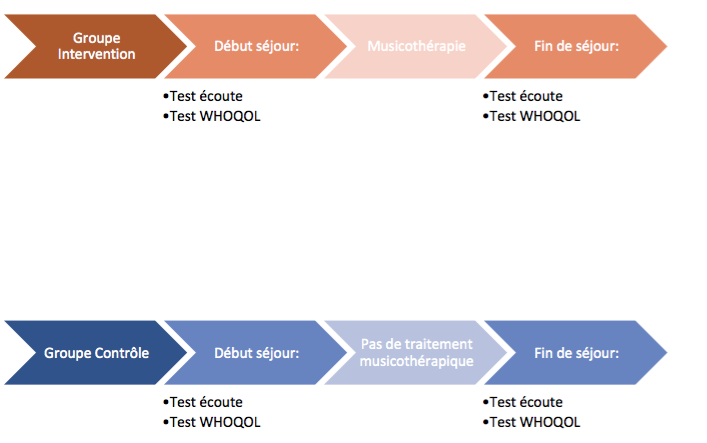
\includegraphics[width=0.7\linewidth]{images/Groupecontrole.png}
\caption[Schéma du déroulement]{Déroulementde l'étude avec les
         deux groupes}
       
\label{groupecontroleimage1}
\end{figure}

\begin{figure}
\centering
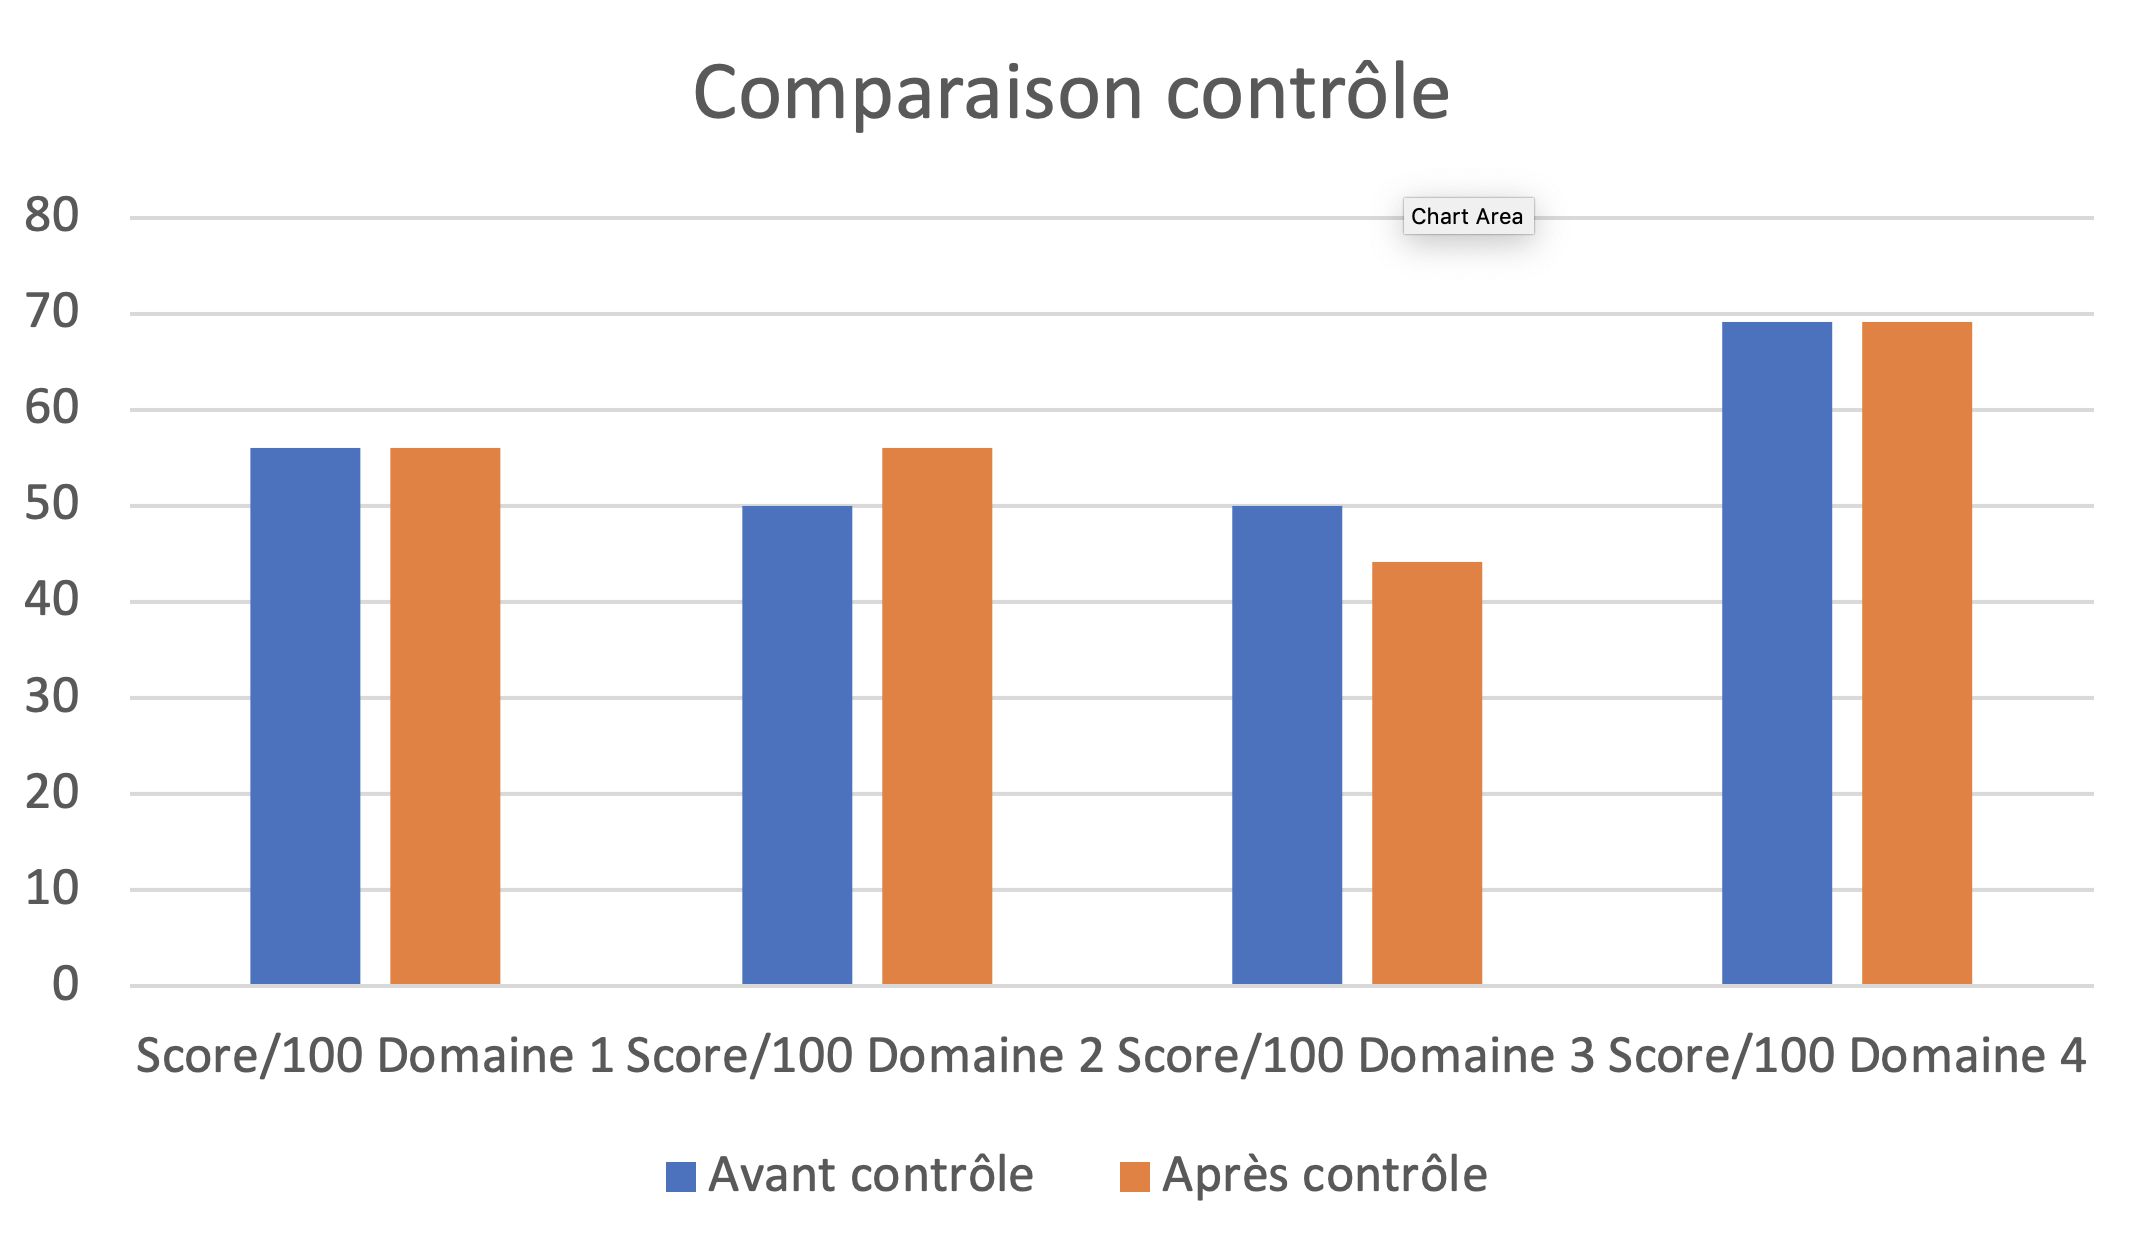
\includegraphics[width=0.7\linewidth]{images/Compcontrole.png}
\caption[Schéma du déroulement]{Déroulementde l'étude avec les
         deux groupes}
       
\label{groupecontroleimage1}
\end{figure}

\begin{figure}
\centering
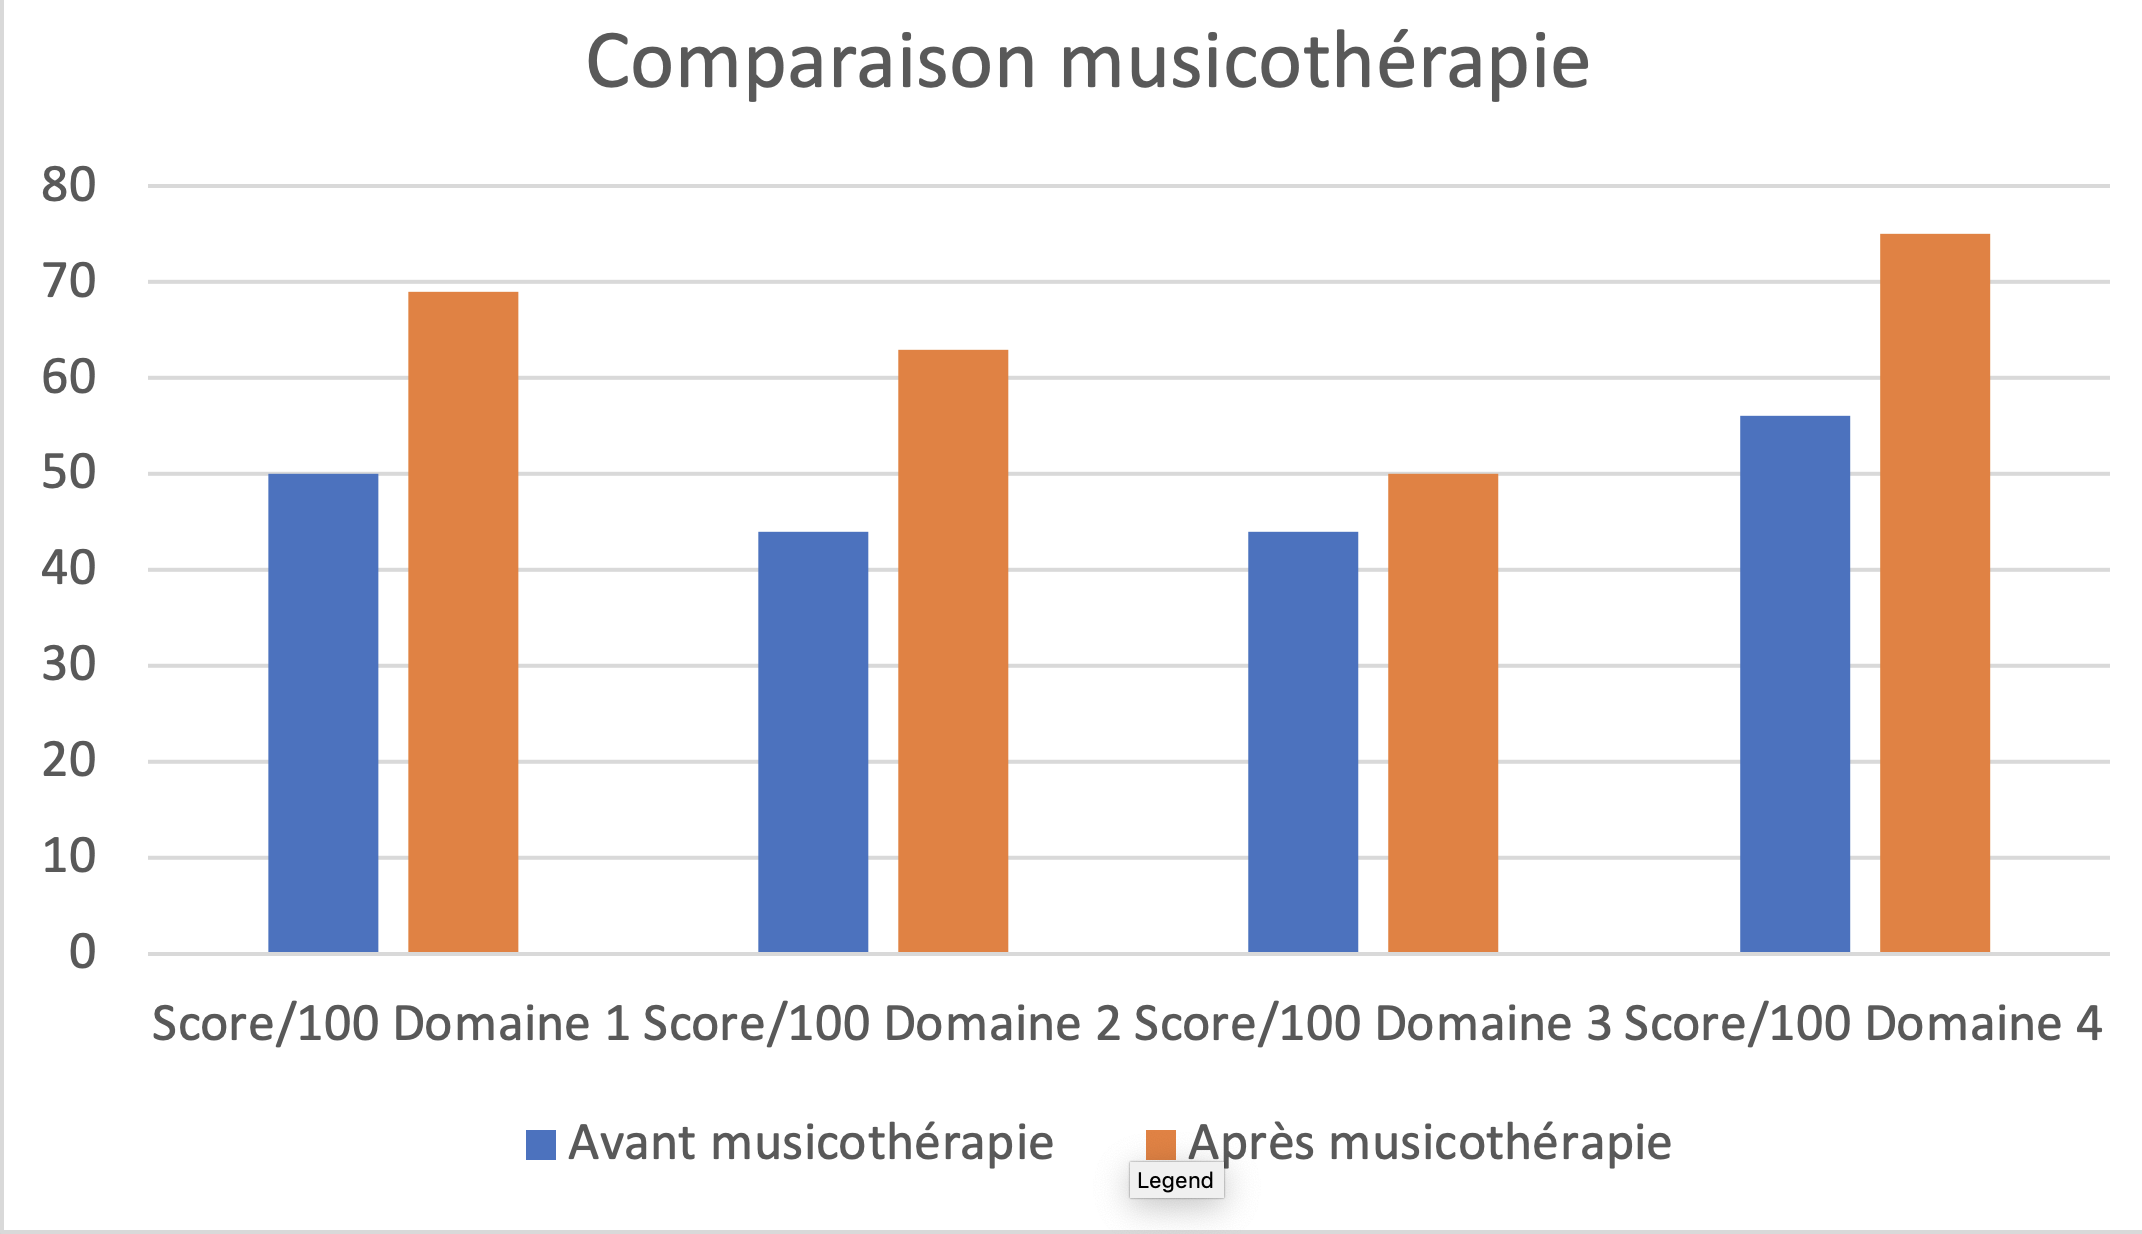
\includegraphics[width=0.7\linewidth]{images/Compmusico.png}
\caption[Schéma du déroulement]{Déroulementde l'étude avec les
         deux groupes}
       
\label{groupecontroleimage1}
\end{figure}



   


\section{Interprétation: les 3 zones de fréquences avec leur résonance en musicothérapie et en
  psychologie}


	Informations croisées avec les informations récoltées par les 3 
          zones du test d'écoute:
          
Les paramètres utilisés en musicothérapie trouvent leur lien avec les
3 zones de fréquences d'interprétation psychologique du test d'écoute.
\begin{itemize}
 \item Le rythme, tempo, puls  =  Z.1: le physique, le corps, l'incorporéisation et
l'intégration du rythme,
la posture d'écoute.

\item La voix, le timbre, la mélodie =  Z.2:  l'expression vocale, la communication,
l'émotionnel, la sensibilité, l'affect.

\item La justesse= l'harmonie (consonance, dissonance) et l'improvisation = Z.3:  la créativité, l'interprétation, la
résonance, la musicalité, la motivation, le non-verbal (
l'intraduisible en mot), l'espace.
\end{itemize}

Si nous référons à la conception antique des chakras ainsi qu'au sens de la
topique de Freud (ça, moi et surmoi), nous trouvons des correspondances
avec les trois zones entre les
fréquences et ``la distribution de l'énergie pulsionnelle'' ou entre
les 
``caractéristiques du son et l'énergie instinctuelles''. (B.Auriol, La
clef des sons).
``La mélodie est la seule forme musicale de la décharge individuelle, car le rythme est le moteur, pré-musical, et l'harmonie, supra-individuelle `` (Mosonyi, 1935, cité par Michel, 1965).

 

\begin{figure}
	\centering
	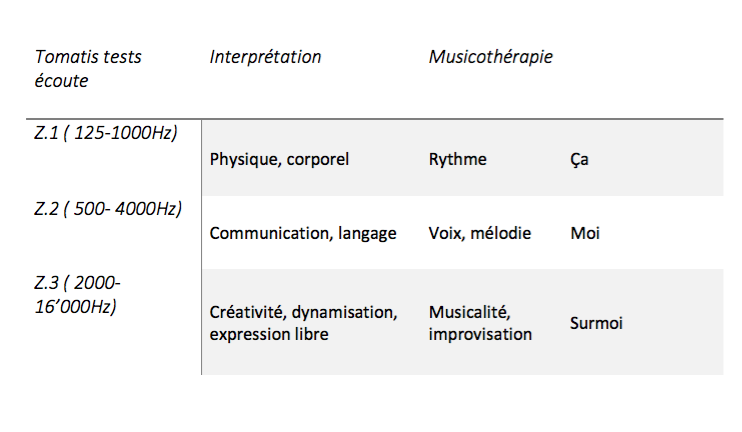
\includegraphics[width=0.7\linewidth]{images/testinterpmusico}
	\caption[ L'interprétation des 3 zones et leur correspondance
        en musicothérapie]{Graphique. interprétation des 3 zones du
          test et leur correspondance en musicothérapie}
       
	\label{graphiquecolonnetestmusico}
      \end{figure}











      


  

\section{Comparaison de deux tests d'écoute, avant et après la musicothérapie: 1°Test--2°test, considérations générales}
	
 	
\subsection{Le patient M avant musicoth.}

 	Le patient M souffre de Burnout. Vif, il se montre très
        intéressé pour participer à l'étude.
 
 	
 	\begin{figure}[tbh]
 		\centering
 		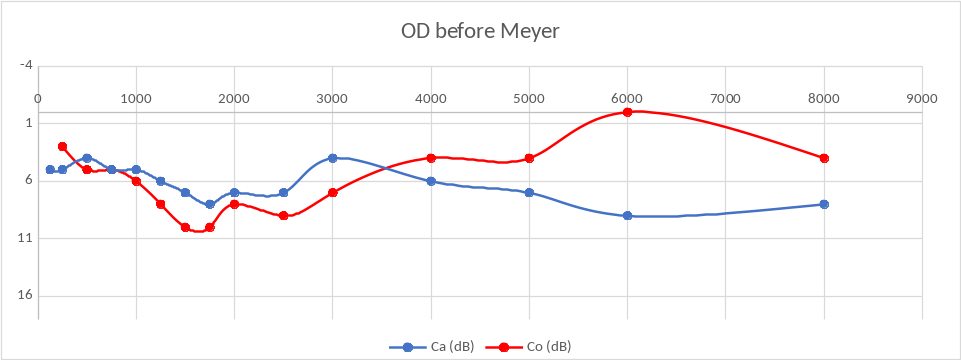
\includegraphics[width=0.7\linewidth]{images/clinique/od_before_meyer.png}
 		\caption{Test d'écoute avant musicothérapie}
 		\label{fig:odbeforemeyer}
 	\end{figure}
 	
 	\lipsum[1]
 	
 	
 	
 	
 	\begin{figure}
 		\centering
 		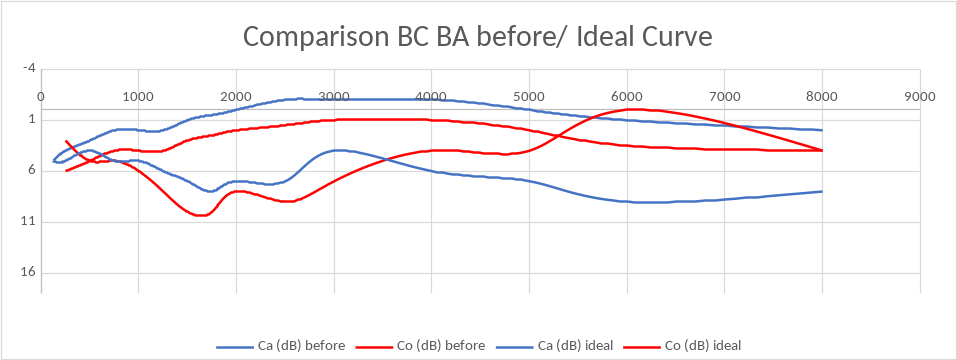
\includegraphics[width=0.7\linewidth]{images/clinique/comparison_bc_ba_before_vs_ideal_curve_meyer.png}
 		\caption[Comparaison avec la courbe idéale]{Comparaison avant
                  musicothérapie des
                  courbes  avec la courbe idéale}
 		\label{fig:comparisonbcbabeforevsidealcurvemeyer}
 	\end{figure}
 	
 	
 	\subsection{Le patient M après la musicoth.}
 	\lipsum[1]
 	\begin{figure}[h]
 		\centering

 		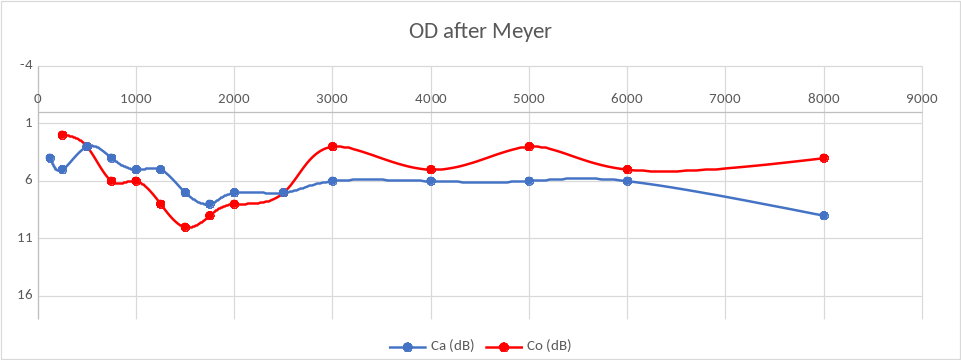
\includegraphics[width=0.7\linewidth]{images/clinique/od_after_meyer.png}
 		\caption{Test d'écoute après la musicothérapie}
 		\label{fig:odaftermeyer}
 	\end{figure}
 
 \lipsum[1]
 
 \begin{figure}[bh]
 	\centering
 	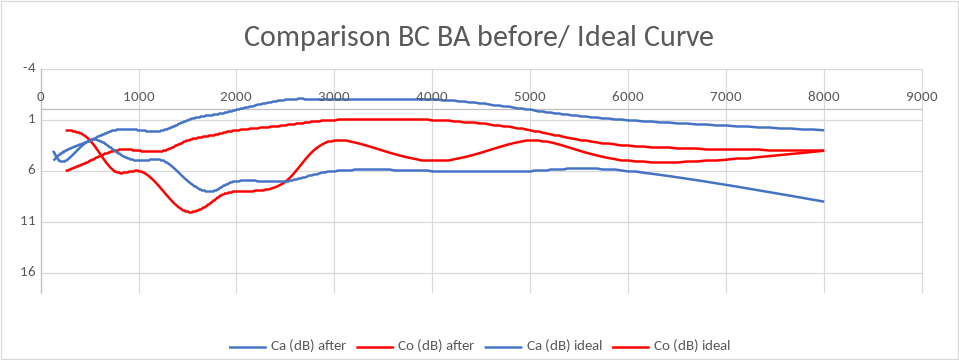
\includegraphics[width=0.7\linewidth]{images/clinique/comparison_bc_ba_after_vs_ideal_curve_meyer.png}
 	\caption{Comparaison avec courbe idéale, après}
 	\label{fig:comparisonbcbaaftervsidealcurvemeyer}
 \end{figure}
 
 





      



 


\section{Graphique:  WHOQO-Bref et Test d'écoute}

Le patient 


\section{Résultats}










   
 

  

  
  


   
   
   
   







\paragraph{Hypothèse}



\paragraph{Y-a-t-il une modification de l'écoute du patient après une prise
en charge en musicothérapie ?}
Est-ce que le processus d'écoute en musicothérapie améliore la capacité
d'écoute ? Devient-elle différente après une musicothérapie?

Est-ce que les test auditifs avant et après la musicothérapie permettent
de visualiser l'action de la musicothérapie?


\paragraph{Est-ce que les résultats ($=$ un changement dans l'écoute) d'une prise
en charge musicothérapeutique peuvent être lisibles et visibles dans
un test d'écoute?}
Est-ce possible d'évaluer un travail musicothérapeutique au moyen
d'un test d'écoute?
Est-ce que ces résultats sont significatifs? 

\paragraph{Est-ce que l'écoute du patient s'est modifié ? si on a pu observer
une modification, dans quel sens va -t-elle ?}

Le contexte: 
est-ce que le contexte est suffisant pour
ressortir des résultats ?





